\label{sec:intro}

The cooperation of agents can expand the capability of an unmanned system [??], and the multi-agent intelligent system is a promising research field.
Multi-robot exploration (MR-Explore) \cite{corah2019communication} provides location and map for each robot . It is the basic task for many multi-robot applications, such as multi-robot navigation [??] and multi-robot rescue[??].

The multi-robot exploration ( MR-Explore ) system \cite{corah2019communication, cieslewski2018data} consists of several robots, which each executes the system illustrated in \Cref{fig:maexp}. Each input frame is fed to the Feature-point Extraction (FE, \textcircled{1}) module for VO. 
And some of the input frames, called key frames, are also fed to the Place Recognition (PR, \textcircled{2}) module.
PR module generates the compact image representation, which produces the candidate place recognition matches between different robots. The VO (\textcircled{3}) based on the feature-points (\textcircled{1}) produces the sparse map and the trajectory that can be used for location. The relative pose ( RelPose ) module dose the same operation as VO(\textcircled{3}) and establishes relative poses between the candidate place matches. The decentralized optimization module (DOpt, \textcircled{4}) and the global map generation module (\textcircled{5}) optimize the  intra-robot relative pose measurements from VO and the inter-robot relative pose measurements from RelPose, and merge the maps. The exploration module (\textcircled{6}) decides an unexplored goal point for each robots to move based on the merged map and the estimated location. The navigation module (\textcircled{7}) navigates each robot to the goal point, including path planning and obstacle avoidance.
In this paper, we optimize the scheduling of PR(\textcircled{2}) and the VO (\textcircled{3}) based on the feature-points (\textcircled{1}) across the CPU side (processing system, PS) and FPGA side (programmable logic, PL) on Xilinx MPSoC \cite{MPSoC}.

% For the keyword \textit{"robot"}, the feature-point extraction (FE) is a fundamental component for the visual odometry to estimate the 6 degrees of freedom (6-DoF) pose [??].
% For the keyword \textit{"multi"}, place recognition (PR) converts the input image into a short representation code, which is a fundamental element to produce candidate place matches between different robots [??].
% Recent works use CNN to extract feature-points \cite{detone2018superpoint, simo2015discriminative, yi2016lift} and generate the representation code \cite{arandjelovic2016netvlad, radenovic2018fine}. 
% The CNN-based feature-points \cite{detone2018superpoint} reaches 10\%-30\% higher matching accuracy compared with the popular handcrafted extraction method, ORB based feature-point extraction \cite{Mur-Artal:2017281}.
% The accuracy of the representation code from another CNN-based method \cite{radenovic2018fine} is also ??\% better than the handcrafted method [??].

\begin{figure}[t]
	\centering
	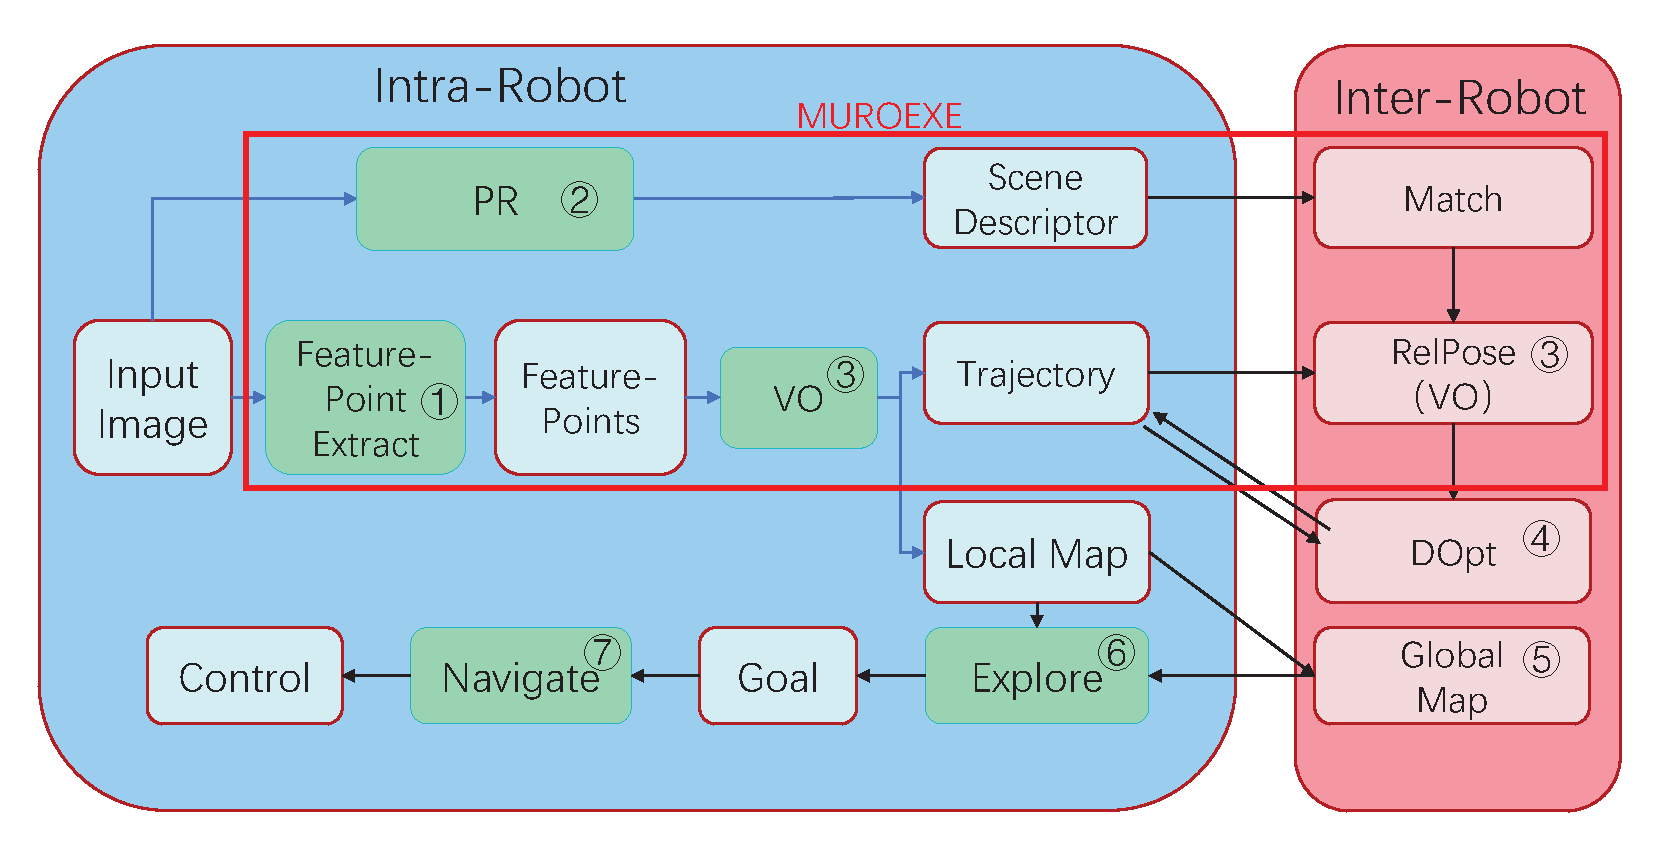
\includegraphics[width=0.99\linewidth]{fig/maexp.eps}
    \caption{
        The components in MR-Explore. \textcircled{1}\textcircled{3} are basic for a single robot, should be execute every frame. \textcircled{2} generates representation code for some key frames. \textcircled{4}\textcircled{5} are only executed when representation codes are matched across robots and they are latency tolerant.  \textcircled{6}\textcircled{7} are for decision and navigation, also latency tolerant.
    }
	\label{fig:maexp}
\end{figure}


% \Cref{fig:maexp} illustrates the computation modules in MR-Explore.
% Feature-point extraction (\textcircled{1}) and visual odometry (VO, \textcircled{3}) should be performed for each input frame, and should be completed before the next frame. 
% Place Recognition (PR, \textcircled{2}) generates the representation code for some key frames, and sends them to other robots. 
% When the  representation codes from different robots are matched, optimization (\textcircled{7}) and map merging ((\textcircled{8})) are performed to merge the trajectories and maps. \textcircled{4}\textcircled{5}\textcircled{6} are for decision-making and navigation based on the merged maps. 



Recent works use CNN to extract feature-points(\textcircled{1} in \Cref{fig:maexp}) \cite{detone2018superpoint, simo2015discriminative, yi2016lift} and generate the representation code (\textcircled{2} in \Cref{fig:maexp}) \cite{arandjelovic2016netvlad, radenovic2018fine}. 
The CNN-based feature-point extraction method, SuperPoint \cite{detone2018superpoint}, reaches 10\%-30\% higher matching accuracy compared with the popular handcrafted extraction method, ORB\cite{Mur-Artal:2017281}.
The accuracy of the representation code from another CNN-based method, GEM \cite{radenovic2018fine}, is also ??\% better than the handcrafted method [??].
Thus, we adopt these CNN methods to realize the Feature-point Extraction and  Place Recognition. 
Besides these two components, more CNN-based methods, such as semantic segmentation \cite{long2015fully} and object detection \cite{ren2015faster}, can be introduced into robots to achieve better accuracy in future.

However, CNNs are computation consuming. A single forward of the CNN-based SuperPoint \cite{detone2018superpoint} feature-point extraction consumes 39G operations \cite{detone2018superpoint}, and a single forward of the CNN-based GEM \cite{radenovic2018fine} place recognition consumes 42G operations \cite{radenovic2018fine}.
% Even if only FE and PR are implemented in CNN, the computational complexity reaches 1 TOP/s , which poses a challenge to the real-time performance of embedded systems.


\begin{figure*}[t]
    % \flushleft
    \centering
	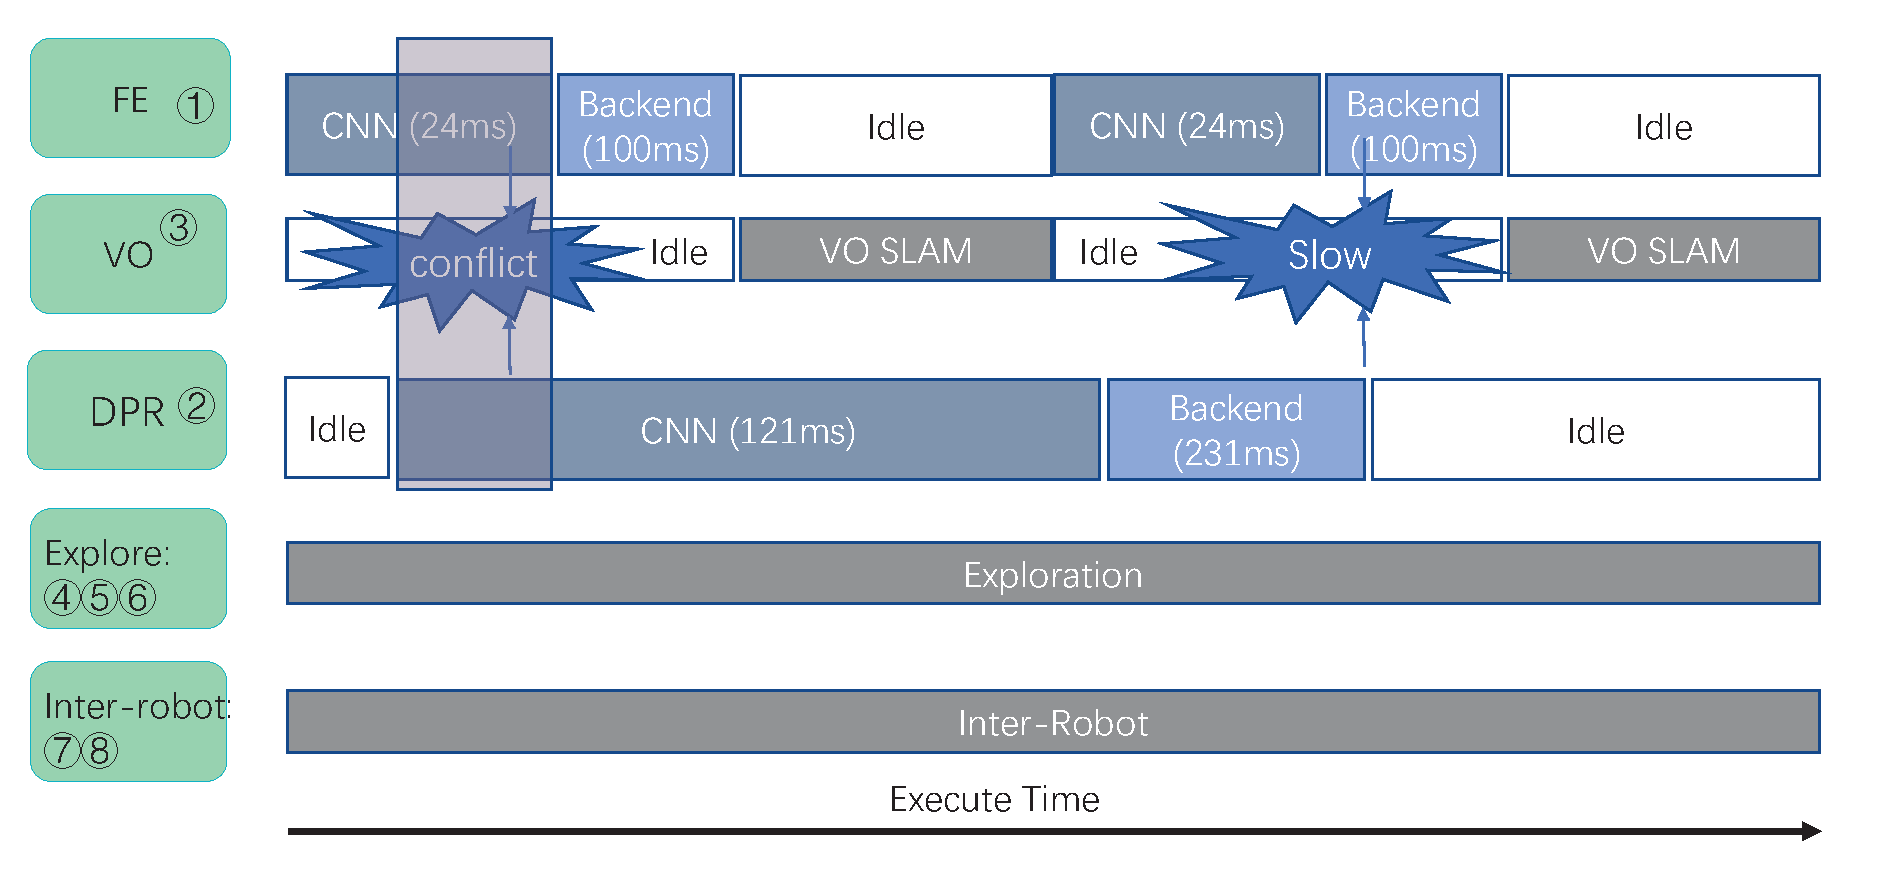
\includegraphics[width=0.99\textwidth]{fig/overalltime.eps} 	
    \caption{
    The overall timeline of MA-Explore.
    }
	\label{fig:overalltime}
\end{figure*}


% In recent years, FPGA is becoming a promising platform for algorithm acceleration. 
To deploy the CNNs on the embedded real-time system, previous works design CNN accelerators on FPGA \cite{guo2017angel,yu2018instruction,li_high_2016,qiu2016going,lu_evaluating_2017}. With the help of network quantization and data reuse, the speed of CNN accelerators on embedded FPGA reaches 3TOP/s \cite{lu_evaluating_2017}.
However, these previous CNN accelerators are designed and optimized to accelerate a specific CNN. They can not automatically schedule two or more tasks simultaneously. 
% The inability of CNN accelerators to support multi-task makes it difficult for researchers in robotics to use embedded FPGA.


We do a simple profiling of MA-Explore with the CNN accelerator. The CNN backbones of FE and  PR are executed on the FPGA accelerator, Angel-Eye\cite{guo2017angel}, and other operations, including the post-processing of the CNN-based FE and PR, runs at the CPU. The timeline of each component is illustrated in \Cref{fig:overalltime}. 
The threads of FE and PR may need to process CNN at the same time, the simultaneous requirements of CNN will lead to hardware resources conflicts in \Cref{fig:overalltime}. The inability of CNN accelerators to support multi-task makes it difficult for researchers in robotics to use embedded FPGA.

In order to facilitate robotic researchers to run different CNN tasks simultaneously on the FPGA accelerators, the accelerator should support the following three features:

\textbf{Multi-thread:} Different components in a robot are from different developers. The Robot Operating System (ROS) \cite{quigley2009ros} is a popular middleware fusing these independent components. Each component in ROS is considered as an independent thread. Different threads should have independent access to the FPGA accelerator without knowing the status of other threads.


% A robot contains many components including perception, decision-making, and control. 
% The Robot Operating System (ROS) \cite{quigley2009ros} is a popular middleware fusing different components from different developers. 
% In ROS, each module is considered as an independent thread on CPU. 
% Different threads should have easy access to the FPGA accelerator.

\textbf{Dynamic Scheduling:} The execution of CNN depends on other operations, like VO module on \Cref{fig:overalltime}. 
These operations are running at CPU, and the execution time varies with the input data [??] (10ms - 50ms for VO). 
The accelerators cannot predict when to start a task. 
Therefore, the FPGA accelerator should be scheduled dynamically to support irregular task requests from the software.

\textbf{Scheduling by priority:} Different components have different priorities. The control and perception tasks usually have higher priorities, while the long-term decision and optimization have lower priorities \cite{RamsauerKLM17}. The critical tasks, which are latency-sensitive,  need to be processed firstly on the accelerator.

The concept of interrupt \cite{jen1974processor} is introduced the CPU in the 1960s, enabling the CPU to support dynamic multi-thread scheduling by priority, thus satisfying these three features on CPU. Therefore, we introduce the concept of interrupt to the CNN accelerator.

Besides the CNN backbone, the post-processing of the CNN-based methods, including normalization, softmax, rank, etc., is also computation consuming. As illustrated in \Cref{fig:overalltime}, the execution time of post-processing for FE on embedded CPU (~60ms) exceeds that of CNN backbone on the accelerator (30ms), and becomes the bottleneck of the system.

To address the above challenges, we propose an INterruptible CNN Accelerator for Multi-robot Exploration (INCAME) for rapid deployment of MR-Explore on FPGA, with following contributions:

\begin{itemize}
    % \begin{itemize}[leftmargin = 10 pt]
\item We propose a CNN-based MA-Explore framework based on FPGA. The hardware and software modules in INCAME is designed for ROS \cite{quigley2009ros}, so that the modules can be easily used in other applications.
\item We propose a \textbf{virtual-instruction-based} interrupt method to make the CNN accelerator support dynamic multi-thread scheduling by priority.
\item We optimize the data flow of the post-processing operations. RTL/HLS modules are designed for the optimized post-processing.
\end{itemize}

The rest of this article is organized as follows: \Cref{sec:relate} will introduce the related work. \Cref{sec:cnninterrupt} details the {virtual-instruction-based} interrupt. \Cref{sec:hardsoftcodesign} details the optimization of post-processing. \Cref{sec:incame} introduces the INCAME framework with ROS. Experimental results and analysis are given in \Cref{sec:experiments}. \Cref{sec:conclusion} concludes this article.